\documentclass[11pt]{article}
\usepackage[margin=0.9in]{geometry}
\usepackage{lmodern,amsmath,booktabs,graphicx,xcolor}
\usepackage[colorlinks=true,urlcolor=teal,citecolor=teal]{hyperref}
\title{Missing sensors change the meaning of model confidence\\\large Participant transfer, dropout training and the cost of refusing a measurement}
\author{James N. Jean IV\\Independent research}
\date{28 October 2026\\GitHub research manuscript; not peer reviewed\\Corrected retrospective evaluation (N1)}
\begin{document}\maketitle
\begin{abstract}
A movement classifier that requests another measurement needs a useful balance between error and refusal. Using public smartphone inertial windows, this study compares clean-only and dropout-augmented training under participant separation. Seventeen declared configurations are selected using six validation participants; the initial evaluation reserved nine source-test participants until selection froze; after a numerical repair, the same test was rescored and is reported as corrected retrospective. The selected augmented logistic model retains 99.5\% of intact windows at 91.0\% accuracy. Under accelerometer loss it retains 63.9\% at 82.0\% accuracy, and under gyroscope loss 99.3\% at 84.6\%. Thus the validation target of 90\% retained-window accuracy fails to transfer to both missing-sensor conditions. Dropout training improves useful coverage but cannot make a pooled confidence threshold reliable for every failure pattern. The practical next experiment is independent, condition-specific calibration on new participants, with an explicit request for another measurement when the supported operating conditions are absent.
\end{abstract}

\section{The measurement decision}
An activity estimate can be wrong, or the system can decline to provide one. The second outcome also has a cost: a user or operator may need to repeat a recording. Ordinary accuracy hides this tradeoff, particularly when an input stream disappears. This study asks whether training with missing modalities and selecting a confidence cutoff can preserve reliable coverage for people excluded from fitting.

The question builds on the public smartphone activity benchmark introduced by Anguita and colleagues \cite{data,paper}. The contribution is a reproducible comparison of participant transfer, controlled sensor loss and a fixed refusal policy within that established task.

\section{Source, split and intervention}
The UCI archive contains preprocessed accelerometer and gyroscope windows for six instructed activities. Each window has 128 samples at 50 Hz and overlaps its neighbor by 50\%. We use the nine body-acceleration, total-acceleration and angular-velocity axes, anonymous participant identifiers and labels. Video, demographic records and the source's 561-feature table are excluded. The source is CC BY 4.0; the public package retains attribution and exact compressed and original hashes for 24 files.

The official training partition contains 7,352 windows. Participants 3, 8, 15, 22, 27 and 30 supply 2,030 validation windows; the other 15 participants supply 5,322 fitting windows. The official test partition supplies 2,947 windows from nine different participants. Windows never cross participant partitions. The original test source was processed after selection froze; corrected N1 coefficients were committed before retrospective rescoring; overlapping windows are never treated as independent participants.

For each axis, we compute mean, population standard deviation, root mean square, range and mean absolute adjacent difference. Forty-five summaries and two modality-presence indicators enter the experiment. Features describe the full source window; no real-time availability or latency claim is made for the source's upstream filtering.

Every window is evaluated intact, with both total- and body-acceleration features removed, and with angular-velocity features removed. Missing features are set to zero and their modality flag is changed. Removing derived body acceleration together with total acceleration prevents an artificial second accelerometer from surviving the intervention. These are simulated failure conditions imposed on measured data, not observed failures. If both modalities are absent, the policy must abstain regardless of model confidence.

\section{Optimization and protected evaluation}
The declared search contains a training-prior baseline, eight logistic configurations and eight random-forest configurations. Logistic C is 0.01, 0.1, 1 or 10; each value is fitted on clean windows or all three conditions. Forests use 160 trees, depth 8 or 16, minimum leaf size 5 or 20, and the same training alternatives. The seed is 20261028. Forests use bootstrap sampling and square-root feature subsampling. The original L-BFGS-B logistic fit used tolerance $10^{-4}$ and passed a loose stopping rule but failed cross-platform replay. N1 uses Newton-Cholesky for the same L2 multinomial objective, tolerance $10^{-12}$ and at most 100 iterations. The C grid, source split and threshold choices remain fixed. All original results and failures are preserved.

Each fitting participant receives equal total sample weight. Augmented copies share that participant's weight. Logistic scaling is fitted only on fitting rows. Initial validation exposed a numerical warning on constant presence indicators; exactly constant fitting columns are removed before scaling. The original results and warning are retained. No test result informed this correction.

The weighted fitting objective is
\[
L(B,b)=\frac{1}{W}\sum_i w_i\left[\log\sum_c e^{x_i^\top B_c+b_c}-(x_i^\top B_{y_i}+b_{y_i})\right]+\frac{\|B\|_F^2}{2CW},\quad W=\sum_iw_i .
\]
Its Hessian is a nonnegative weighted sum of softmax class-covariance outer products plus the L2 penalty. Intercepts are unpenalized and have a common-shift gauge. Independent checks reconstruct all eight logistic objectives, scalers, probabilities, gradients, Hessian eigenvalues and directional finite differences. The largest final gradient is $2.17\times10^{-13}$, below the $10^{-10}$ gate. Numerical convex-optimization evidence does not establish generalization.

A fitting/validation-only probe found original gradients near $10^{-4}$ versus roughly $10^{-16}$ with the tighter solver, including changed validation predictions. No test outcome selected the repair. Corrected coefficients froze at \texttt{75d7b829b57e33249ff651a70ca3ce86bc004a2f} before rescoring. Test inference reuses these coefficients rather than refitting. The test had already been inspected; this is a corrected retrospective comparison.

Selection maximizes macro F1 averaged across participant-condition groups, with candidate-name tie breaking. This prevents participants with more windows from dominating the selection objective. The selected model is dropout-augmented logistic regression with C=10, the boundary of the tested grid. The clean-only comparator has C=0.1. All 17 candidate scores, times, configurations and validation probabilities are retained. A finite search does not establish a global optimum.

For each selected model, nine maximum-probability cutoffs are evaluated on validation. The rule chooses maximum pooled coverage subject to at least 90\% selective accuracy and 100 retained windows. The resulting cutoffs are 0.5 for the augmented model and 0.95 for the clean-only comparator. Threshold selection calibrates a decision rule, not the probabilities themselves; Brier score, log loss and reliability summaries assess the latter separately.

\begin{figure}[ht]\centering
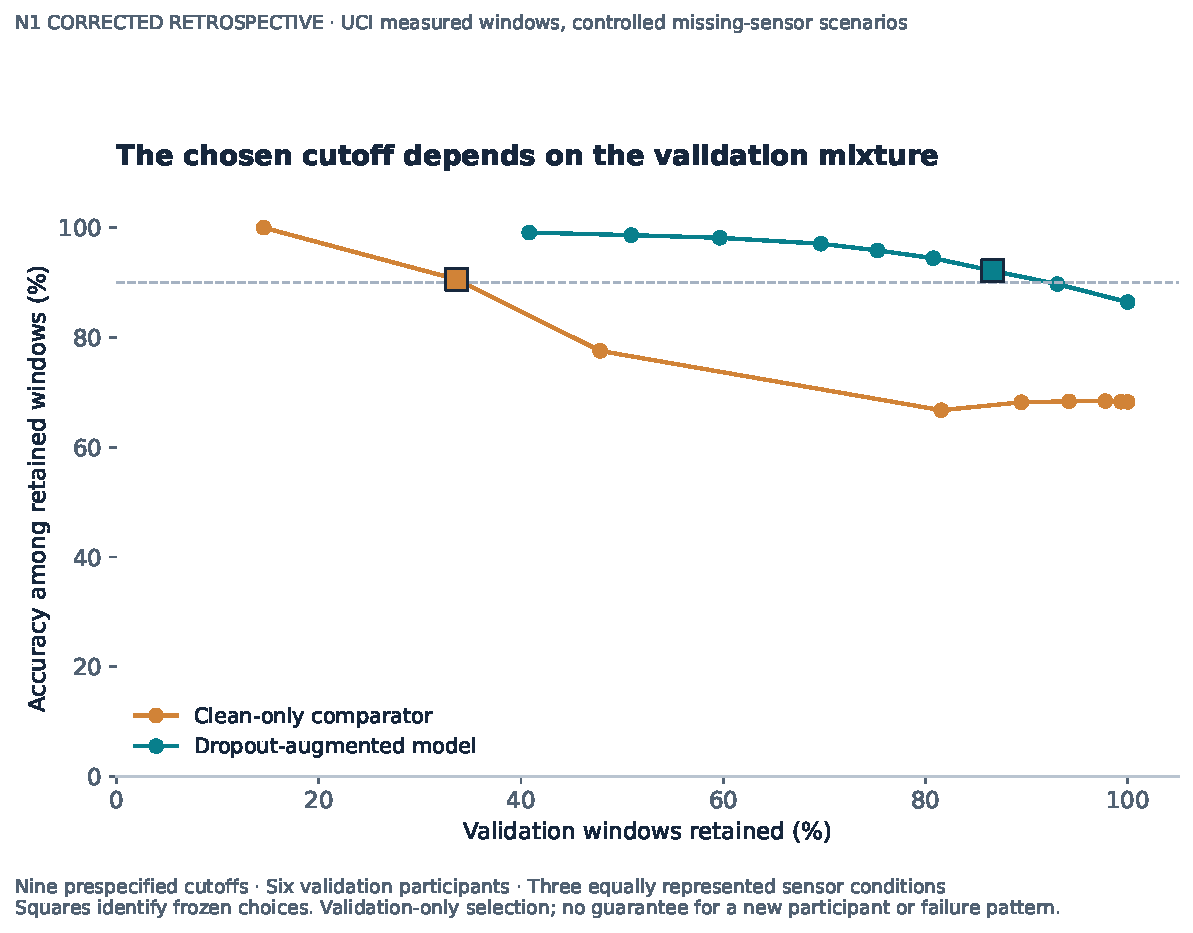
\includegraphics[width=.9\linewidth]{images/abstention-frontier.pdf}
\caption{Validation confidence choices and the retained-measurement tradeoff. The condition mixture is controlled and does not represent observed device-failure prevalence.}
\end{figure}

\section{Results and operating implications}
\begin{table}[ht]\centering
\caption{Frozen policy on previously unseen participants. Coverage and selective accuracy are percentages; Brier is the mean sum of squared six-class probability errors.}
\begin{tabular}{lrrrr}\toprule
Condition & Raw accuracy & Coverage & Selective accuracy & Brier\\\midrule
Intact & 90.7 & 99.5 & 91.0 & 0.139\\
Accelerometer absent & 72.1 & 63.9 & 82.0 & 0.410\\
Gyroscope absent & 84.2 & 99.3 & 84.6 & 0.230\\\bottomrule
\end{tabular}\end{table}

The augmented model improves raw classification under every tested sensor condition relative to the clean-only comparator. Its retained-window accuracy falls below the validation target in both missing-modality conditions. Training robustness and a successful pooled validation constraint do not guarantee reliable selective predictions after participant transfer.

The clean-only comparator retains 45.5\% of intact windows at 98.7\% accuracy and 33.8\% of gyroscope-missing windows at 98.0\% accuracy. With the accelerometer missing it retains 10.8\% at 0.0\% accuracy: all 317 accepted windows are wrong. The earlier incomplete fit reported 178. A high confidence cutoff therefore does not reliably recognize this input failure. Preserving a small but confidently wrong subset is worse than its low coverage alone suggests.

Across the controlled mixture, paired participant-block resampling gives a 95\% interval of 17.1--23.1 percentage points for the augmented model's raw-accuracy improvement and 54.0--60.5 points for coverage improvement. Accepted-correct fraction improves by 45.4--53.4 points. These are conditional intervals from 2,000 resamples of nine participants; they do not establish population or device transfer, nor do they account for a natural failure-frequency distribution.

\begin{figure}[ht]\centering
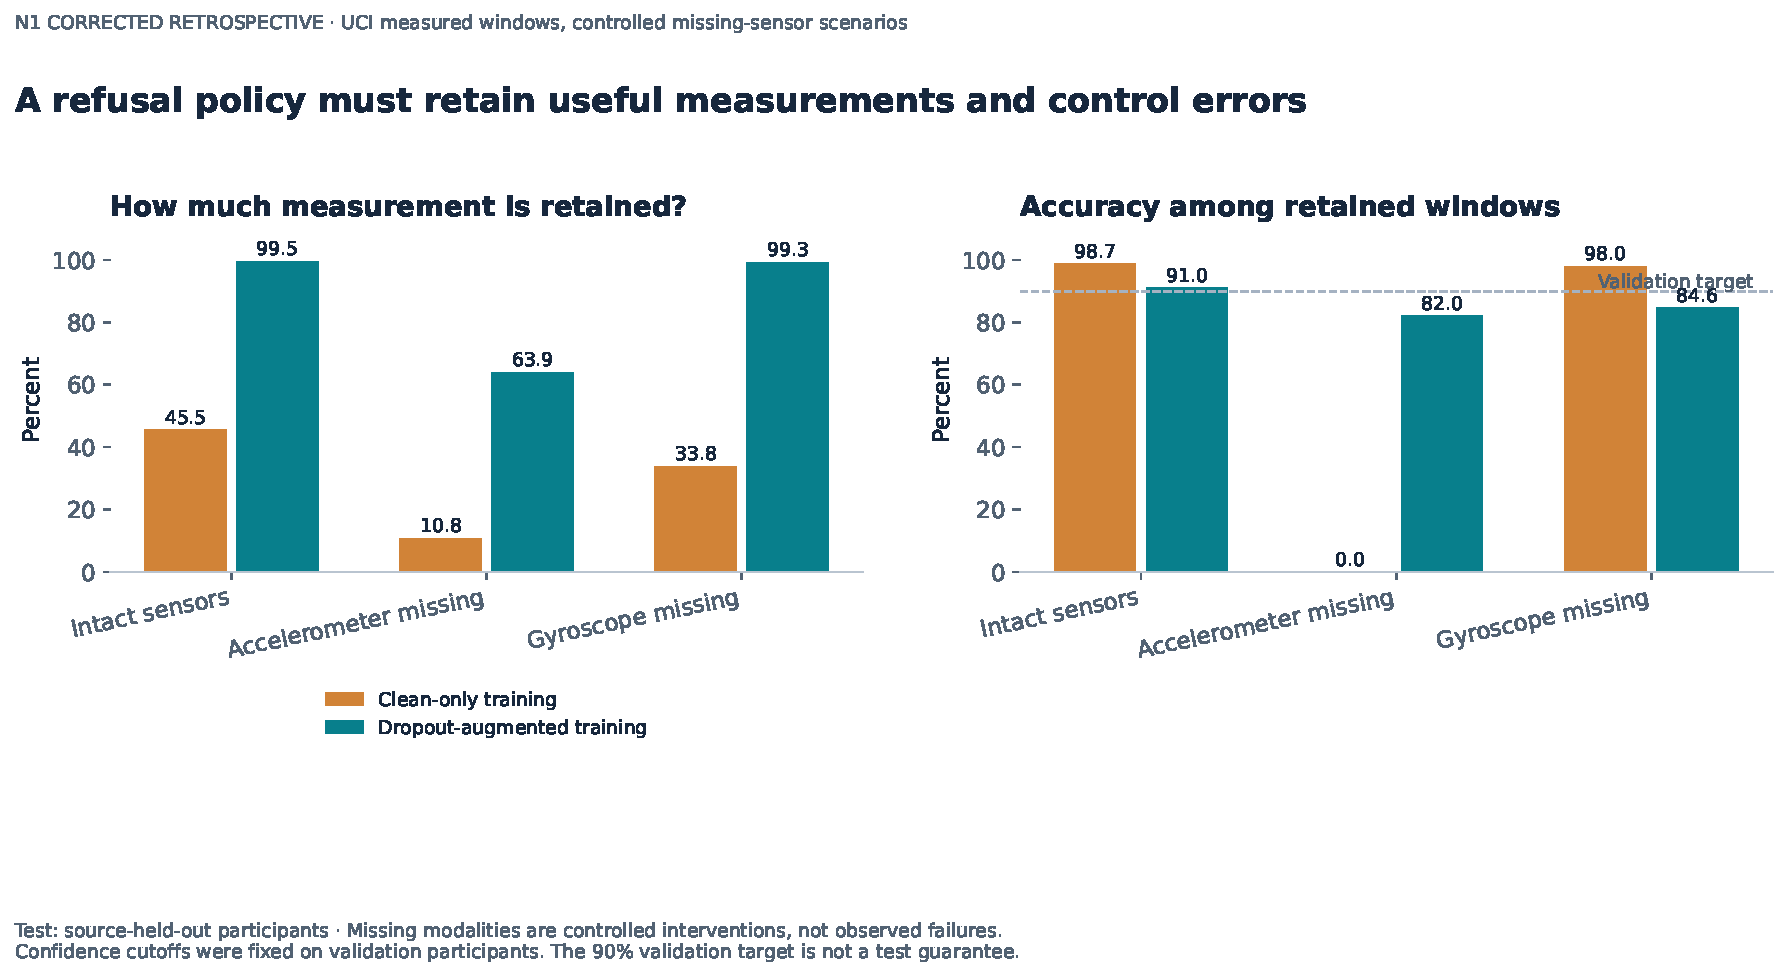
\includegraphics[width=\linewidth]{images/decision-summary.pdf}
\caption{More retained measurements can accompany lower reliability. The fixed validation target does not transfer to all test conditions.}
\end{figure}

\section{Checks, limits and next experiment}
An independent verifier imports no fitting or metric helpers. It recomputes confusion-derived macro F1, accuracy, Brier score, log loss, threshold selection and participant-block intervals from exported probabilities. All source hashes and row identifiers reconcile; feature arithmetic is independently spot checked at 14 boundary/interior windows per source partition. Eight contract tests cover modality lineage, absent-input abstention, participant weights, threshold boundaries, frozen-model identity, label-independent inference and stable extreme logits. A fresh offline replay refits all 17 candidates and checks all coefficients, validation/test probabilities, selections and metrics at the original $10^{-7}$ relative/$10^{-9}$ absolute tolerance. The corrected Windows replay passes; a clean exact-head Linux replay is a separate release gate.

The first test-score export failed because two metric dictionaries both contained a count field. The prediction export had already been saved, but performance metrics had not been inspected. That earlier repair scored its retained predictions without changing a model, feature or cutoff. N1 later refits the same objective to tighter convergence; it preserves earlier outputs and does not present the reused test as untouched. The failure record and prediction hash remain in the public evidence. This repaired computation is reported transparently rather than presented as a new independent test.

The selected systems differ in augmentation and tuned C. Augmented row counts also change effective L2 penalty at fixed C; this comparison does not isolate an augmentation-only causal effect. A matched-penalty ablation on a new cohort is future work.

The source has few participants, one device configuration, instructed activities and processed overlapping windows. Synthetic sensor removal is a controlled stress test and cannot establish behavior under hardware faults, interrupted timing or unfamiliar tasks. Participant transfer remains difficult even after augmentation. The next experiment should collect a new participant cohort with measured failure patterns, prespecify condition-specific coverage and error requirements, and test calibration there. Until that evidence exists, a system should request another measurement when its available sensor condition is outside its validated operating range.

\section*{Reproducibility and authorship}
Public source excerpts, code, configurations, prediction exports, figures and checks are at \href{https://github.com/S3R3Bii/sensor-loss-abstention}{the study repository}. This research manuscript is shared on GitHub and has not been peer reviewed. AI assisted coding and drafting; measured results, experimental assumptions and proposed future work are distinguished throughout.
\begingroup\small\begin{thebibliography}{9}\setlength{\itemsep}{2pt}
\bibitem{data} J. Reyes-Ortiz, D. Anguita, A. Ghio, L. Oneto and X. Parra. Human Activity Recognition Using Smartphones. UCI Machine Learning Repository, 2013. \url{https://doi.org/10.24432/C54S4K}.
\bibitem{paper} D. Anguita, A. Ghio, L. Oneto, X. Parra and J. L. Reyes-Ortiz. A Public Domain Dataset for Human Activity Recognition Using Smartphones. European Symposium on Artificial Neural Networks, 2013. Source bibliography and preprocessing documentation accompany the UCI dataset.
\end{thebibliography}\endgroup\end{document}
